\hypertarget{cv:gestionarEntidades}{\section{Gestionar Entidades}} \label{sec:GestionarEntidades}

	Esta funcionalidad le permitirá las acciones necesarias para controlar las entidades asi como sus atributos y visualizarlos en una tabla en el proyecto sobre el que se está operando y solicitar el registro de uno nuevo.

		\subsection{Procedimiento}

			%Pasos de procedimiento
			\begin{enumerate}
				
			\item Ingrese a un proyecto existente desde la pantalla \ref{fig:GestionarProyectosColaborador}.
	
			\item Seleccione la opción \textbf{Entidades} del menú \ref{fig:MN-LPC}.
	
			\item Se mostrará la pantalla \ref{fig:GestionarEntidades} ''Gestionar Entidades''.

			%Pantalla
			\begin{figure}[h!]
				\begin{center}
					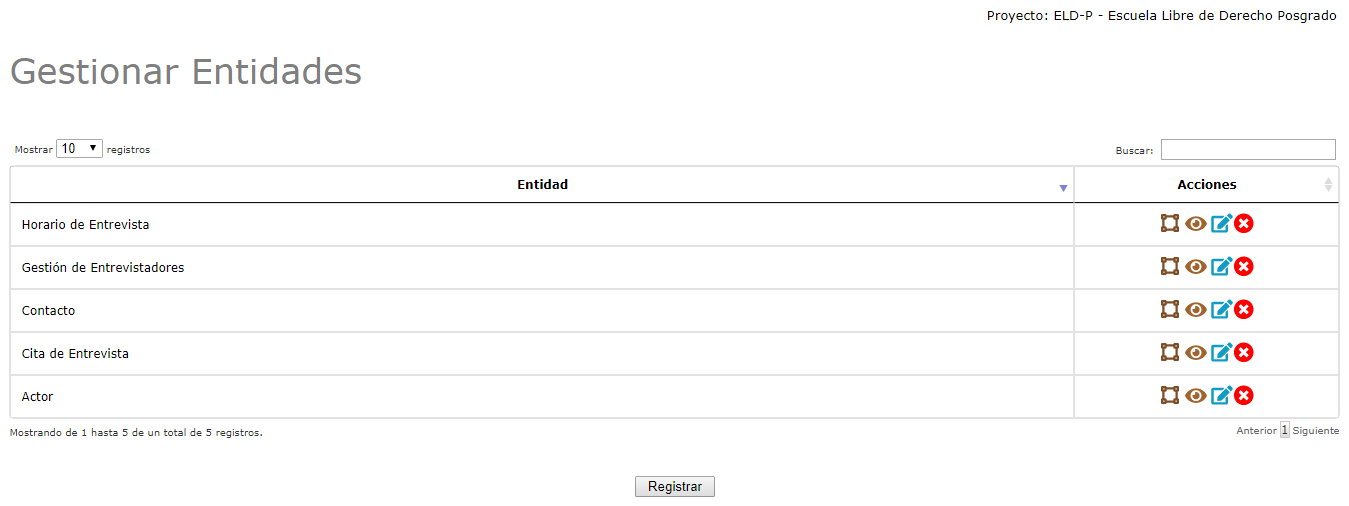
\includegraphics[scale=0.5]{roles/lider/entidades/pantallas/IU12gestionarEntidades}
					\caption{Gestionar Entidades}
					\label{fig:GestionarEntidades}
				\end{center}
			\end{figure}
		
				\item Seleccione la operación que desea realizar:
			
			Para (\hyperlink{cv:registrarEntidad}{Registrar}) dé clic en el botón \IURegistrar.
			
			Para (\hyperlink{cv:modificarEntidad}{Modificar}) dé clic en el icono \IUEditar{} de alguna entidad ya registrada.
			
			Para (\hyperlink{cv:eliminarEntidad}{Eliminar}) dé clic en el icono \IUBotonEliminar{} de alguna entidad ya registrada.
			
			Para (\hyperlink{cv:consultarEntidad}{Consultar}) dé clic en el icono \IUConsultar{} de alguna entidad ya registrada.
			
			Para (\hyperlink{cv:gestionarAtributos}{Gestionar los atributos}) dé clic en el icono \IUAtributos{} de alguna entidad ya registrada.
			\end{enumerate}